\section{Floating point numbers}
\subsection{Definition}
\begin{frame}{Floating point numbers}

\begin{itemize}
    

\item <1->  $x = s.M.\beta^{e-p+1}$ with $s$ the \textbf{sign}, $M$ the \textbf{mantissa} ($\lvert M \rvert \le \beta^p-1)$, $\beta$ a \textbf{base}(\textbf{radix}), $e$ the \textbf{exponent} and $p$ the \textbf{precision}. 
  
\ \\ 
 
\item <2->  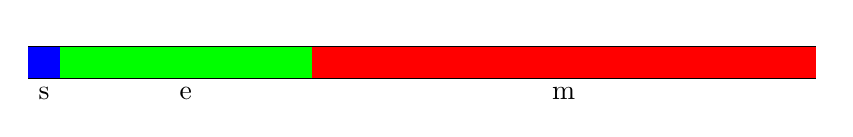
\begin{tikzpicture}
      \draw[step=0.4cm, black,  thin] (0, 0) grid (10, 0.4);   
     \fill [blue](0,0) rectangle(0.4,0.4);
     \fill [green](0.4,0) rectangle(3.6,0.4);
     \fill [red](3.6,0) rectangle(10,0.4);
     \draw (0.2,0) node[below] {s}  ;
     \draw (2,0) node[below] {e}  ;
     \draw (6.8,0) node[below] {m}  ;
     \draw (10,0.4) node[above]{};
\end{tikzpicture}
 \item <3->  \begin{table}[]
      \centering
      \begin{tabular}{|c|c|c|c|}
      \hline
      
        Format &  $Sign$ &  $Exponent$ & $Mantissa$\\
        \hline
         $binary32$& $1$ bit & $8$ bits & $24$ bits\\
         \hline
        $binary64$ &$1$ bit  & $11$ bits &  $53$ bits\\ 
        \hline
         $binary128$ &$1$ bit &  $15$ bits  &  $113$  bits\\
         \hline
        \end{tabular}
        
      \end{table}
      \end{itemize}
\end{frame}

\begin{frame}[Rounding modes]
\begin{itemize}
    \item <1-> \textbf{RNDN}: 
    \begin{itemize}
        \item \textbf{Ties to even}
         
        \item \textbf{Ties to away}
       
    \end{itemize}
    \item <2->\textbf{RNDZ}
    \item <3->\textbf{RNDU}
    \item <4->\textbf{RNDD}
\item <5->
\begin{table}[hbtp]
        \centering
    $$\begin{tabular}{|c|c|c|}
    \hline
    Real Number & +140.8215064611465 & +665.5752955525412\\
    \hline
    RNDN(Ties to even) & +140.821506461146 & +665.575295552541\\
    \hline
    RNDN(Ties to away) & +140.821506461147 & +665.575295552541\\
    \hline
    RNDZ & +140.821506461146 & +665.575295552541\\
    \hline
    RNDU & +140.821506461147 & +665.575295552542\\ 
    \hline
    RNDD & +140.821506461146 & +665.575295552541\\
    \hline
    \end{tabular}$$
\end{table}
\end{itemize}
\end{frame}

\begin{frame}
    \begin{itemize}
    \item  $+0$ and $-0$
    \item $-\infty$ and $+\infty$
    \item NaN 
    \item \textbf{Subnormal} 
    \item   \textbf{Overflow} 
    \item \textbf{Underflow}  
\end{itemize} 
\end{frame}
\begin{frame}
\begin{itemize}
    \item <1-> 
\begin{defin}[\textbf{ulp(x)}]  
 Let $x$ a \textbf{floating-point} number, $x = d_0d_1d_2d_3d_4...d_{p-1}\beta^e$. we therefore have an error to represent it :$\lvert d_0d_1d_2d_3d_4...d_{p-1} - \frac{x}{\beta^e} \rvert $ which is the unit of the last place.
\end{defin}
\item <2->
    \begin{coroll}
If $x$ is a \textbf{floating-point} number, $d_0 = 1$ and that its base is $2$, then we have :
$$ulp(x) \le 2^{-52} \lvert x \rvert$$.
\end{coroll}
\end{itemize}
\end{frame}

\subsection{Necessary tools}
\begin{frame}{Property}

\begin{prope}
 If $X = RNDN(x)$ $\Rightarrow$ $\vert X - x \rvert \le \frac{1}{2}ulp(x)$
\end{prope}

\begin{prope} 
If $X = RNDN(x)$ $\Rightarrow$ $\vert X - x \rvert \le \frac{1}{2}ulp(X)$
\end{prope}

\begin{prope}  
If $X \in \{ RNDD(x), RNDU(x), RNDZ(x), RNDN(x)\} $ $\Rightarrow$ $\vert X - x \rvert \le ulp(x)$
\end{prope}

\begin{prope}
If $X \in \{ RNDD(x), RNDU(x),RNDZ(x), RNDN(x)\} $ $\Rightarrow$ $\vert X - x \rvert \le ulp(X)$
\end{prope}
\end{frame}
\begin{frame}{Unit Roundoff}
$$
    u = \left\{
\begin{array}{ll}
    \frac{1}{2}.ulp(1) = \frac{1}{2}.2^{-52} = 2^{-53}& for \  \ RNDN \\
    \ & \ \\
     ulp(1) = 2^{-52} & for \  \ (RNDU, RNDZ, RNDD)
\end{array}
\right.
$$
\end{frame}

\begin{frame}{\textbf{Sterbenz}’s lemma}
   \begin{lem}[\textbf{Sterbenz}]
In a \textbf{radix-$\beta$} floating-point system with \textbf{subnormal} numbers available, if $x$ and $y$ are finite \textbf{floating-point} numbers such that
$\frac{y}{2} \le x \le 2.y$ , then $x - y$ is exactly representable.
\end{lem} 
\end{frame}
